% 图 7.16 (a) 可公度自旋密度波（q=π/a，自旋逐位反铁磁排列）(b) 不可公度自旋密度波（自旋沿链缓慢旋转）
% 面板标签 (a)(b) 由正文排版提供，图内不重复标注
\documentclass[tikz,border=5pt]{standalone}
\usetikzlibrary{arrows.meta}
\usepackage{amsmath}
\usepackage{bm}
\usepackage{fontspec}
\setmainfont{Times New Roman}
\begin{document}
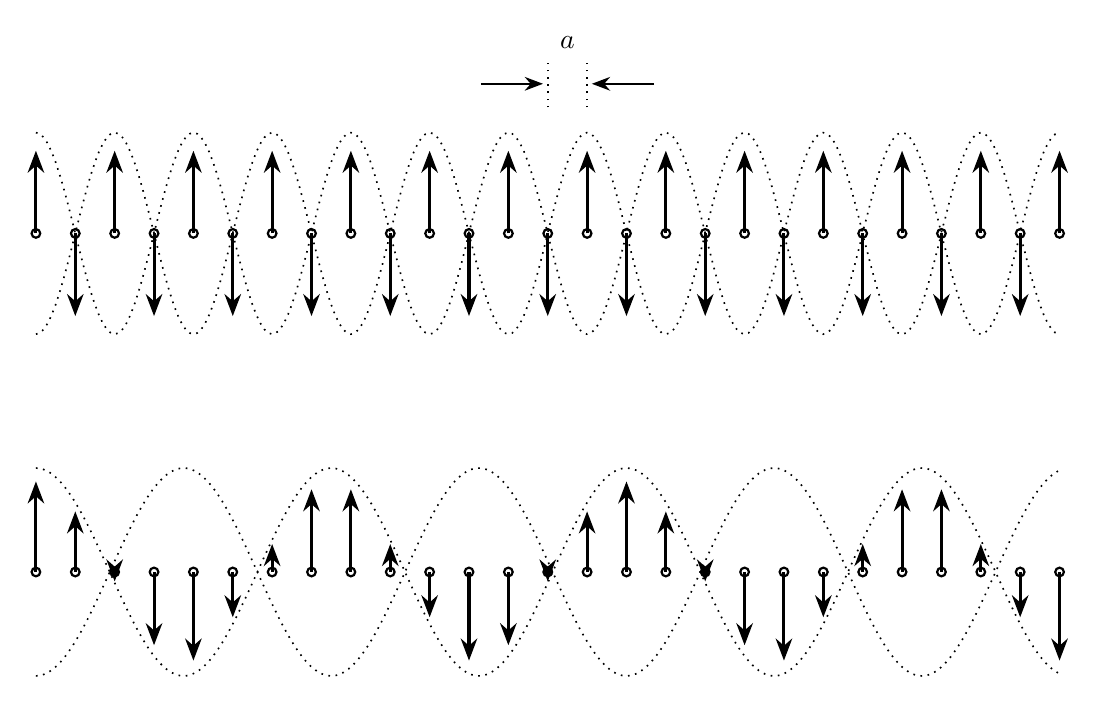
\begin{tikzpicture}[line width=0.8pt,>=Stealth]
% ---------- (a) 可公度 SDW ----------
\begin{scope}
% 上下点状包络：±A|cos(πx/2a)|，a=0.5，A=1.28
\draw[dotted,line width=0.6pt] plot[domain=0:13,samples=261] (\x,{1.28*abs(cos(180*\x))});
\draw[dotted,line width=0.6pt] plot[domain=0:13,samples=261] (\x,{-1.28*abs(cos(180*\x))});
% 原子与自旋箭头（偶位向上、奇位向下）
\foreach \i in {0,...,26}{
  \pgfmathsetmacro\x{0.5*\i}
  \pgfmathsetmacro\L{1.05*pow(-1,\i)}
  \draw[->,line width=1.1pt] (\x,0) -- (\x,\L);
  \draw (\x,0) circle (0.055);
}
% 晶格间距 a 标注（顶部中央）
\draw[dotted,line width=0.6pt] (6.5,1.6) -- (6.5,2.2);
\draw[dotted,line width=0.6pt] (7.0,1.6) -- (7.0,2.2);
\draw[->] (5.65,1.9) -- (6.44,1.9);
\draw[->] (7.85,1.9) -- (7.06,1.9);
\node at (6.75,2.42) {$a$};
\end{scope}
% ---------- (b) 不可公度 SDW ----------
\begin{scope}[shift={(0,-4.3)}]
% 上下点状包络：±A cos(qx)，λ=7.5a
\draw[dotted,line width=0.6pt] plot[domain=0:13,samples=321] (\x,{1.32*cos(96*\x)});
\draw[dotted,line width=0.6pt] plot[domain=0:13,samples=321] (\x,{-1.32*cos(96*\x)});
% 原子与自旋箭头（长度与方向沿链缓慢旋转）
\foreach \i in {0,...,26}{
  \pgfmathsetmacro\x{0.5*\i}
  \pgfmathsetmacro\L{1.15*cos(96*\x)}
  \ifdim\L pt>0.12pt \draw[->,line width=1.1pt] (\x,0) -- (\x,\L); \fi
  \ifdim\L pt<-0.12pt \draw[->,line width=1.1pt] (\x,0) -- (\x,\L); \fi
  \draw (\x,0) circle (0.055);
}
\end{scope}
\end{tikzpicture}
\end{document}
